\section{Exercise 2: Entropy of a random variable from a data series}

\begin{frame}{ Entropy of a random variable from a data series}

In this exercise, our aim is to:
\begin{itemize}
    \item Identify a data series and estimate the probabilities of the outcomes based on
their occurrences, updating the probabilities at each time step.
    \item At each time step, compute the entropy, plot its behaviour, and discuss the results
\end{itemize}
\end{frame}


\begin{frame}{Data Series Overview}
This dataset could be very suitable for our entropy calculation exercise, as it provides a real-world time series that likely exhibits interesting patterns and variations over time. The data is organized as a time series, meaning it's collected at regular time intervals (daily in this case) over a while. We have used Delhi's temperature record for over 4 years.
This is the\href{https://www.kaggle.com/datasets/sumanthvrao/daily-climate-time-series-data}{"link"} to the dataset.

Although the dataset contains other information like date, mean temperature, humidity, wind speed, and mean pressure, we mainly focused on mean temperature and dropped all the rest.
\end{frame}

\begin{frame}{Data Distribution}
The distribution below represents temperature data distribution which shows the frequency of bins, each bar represents a 2°C temperature range, as specified in the code
\begin{figure}
    \centering
    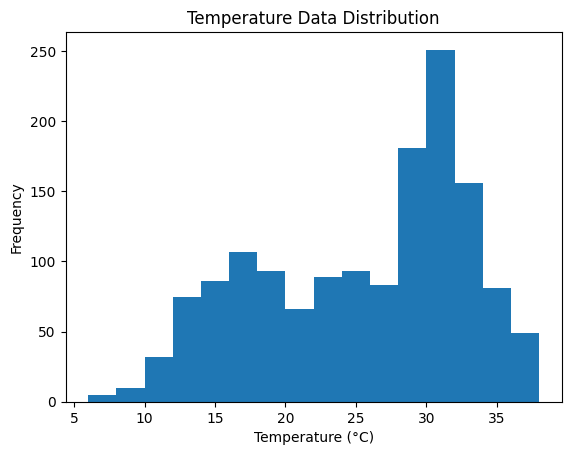
\includegraphics[width=0.5\linewidth]{temp_distribution.png}
    \label{fig:enter-label}
\end{figure}
\end{frame}
\begin{frame}{Probability Estimation}
Binning is necessary to transform continuous temperature data into discrete categories, making it possible to compute the probabilities of the temperature falling within specific ranges. Once the data is binned, the frequency of data points in each bin is counted. These frequencies are then converted into probabilities by dividing each count by the total number of data points at each time step.
These probabilities represent the likelihood of the temperature falling within each bin at a given time. using Shannon’s entropy formula, entropy is computed for each time step based on the probabilities of the data falling within different bins.


Entropy $H(X)$ is calculated based on the following formula derived from Shannon’s work:
\[
H(X) = -\sum_{i=1}^{n} p(x_i) \log_2{p(x_i)}
\]
\end{frame}

\begin{frame}{Iterative Calculation Over Time}
The core of the code involves a loop that recalculates entropy as the dataset grows. At each iteration, the temperature data from day 1 to day "i" (where i is the current time step) is considered.

\begin{figure}
    \centering
    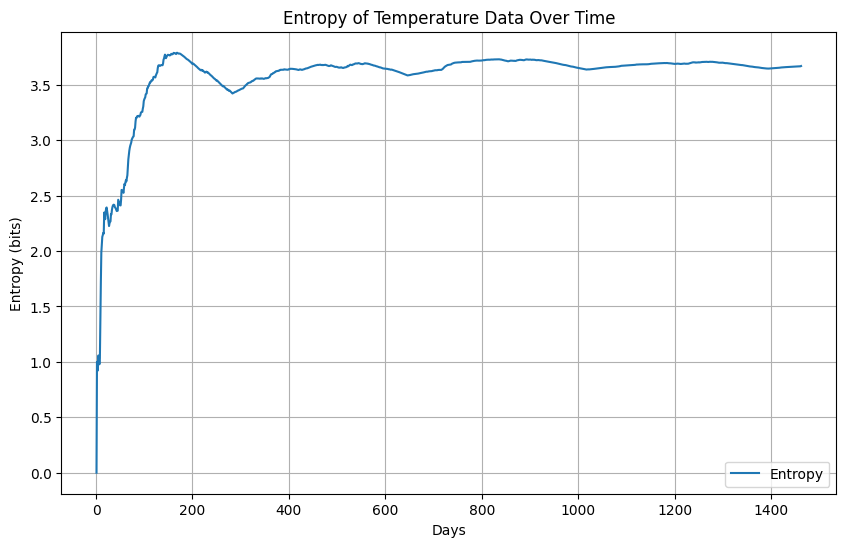
\includegraphics[width=0.5\linewidth]{entropy.png}
    \label{fig:enter-label}
\end{figure}
\end{frame}

\begin{frame}{Result}
The process repeats, recalculating probabilities and entropy at every step, and the results are stored in a list called "entropy values". Finally, the entropy values are plotted against time (days). The x-axis represents the number of days (i.e., how much data has been accumulated), and the y-axis represents the entropy (measured in bits).

At the very beginning (first 50–200 days), the entropy rises sharply. This indicates that the uncertainty in the dataset is increasing rapidly. As more data is introduced, the system is becoming less predictable—likely because more variations in temperature are being captured. After the sharp rise, the entropy curve flattens out and oscillates around a value close to 3.5 bits. This stabilization indicates that the system has reached a point where additional data does not significantly increase uncertainty. In other words, the temperature data has become more predictable, and no new significant randomness is being introduced.
\end{frame}
\begin{frame}{Result}

The plot suggests that the temperature dataset initially had a lot of variability, but as more data was accumulated, the variability reached a limit. This pattern is common in systems where initial observations are more uncertain but then start to follow a more predictable pattern as the dataset grows.
\end{frame}